\documentclass[12pt,a4paper]{report}

\usepackage{url}
\usepackage{graphicx}
\usepackage{listings}
\usepackage{xcolor}
\usepackage{amsmath}

\begin{document}

\chapter{Hodgkin-Huxley Model}

\section{Introduction}

The Hodgkin-Huxley model, proposed by Sir Alan Hodgkin and Sir Andrew Huxley in 1952, revolutionized the field of neuroscience by providing a quantitative understanding of the generation and propagation of action potentials in neurons. This mathematical framework emerged from a decade-long collaboration between Hodgkin and Huxley, culminating in the publication of their landmark papers in the Journal of Physiology.

\subsection{Historical Background}

The Hodgkin-Huxley theory emerged as a result of a remarkable collaboration between Hodgkin and Huxley from the late 1930s to the early 1950s. Their work was informed by several key experimental findings. Cole and Curtis demonstrated that the action potential is associated with a significant increase in membrane conductance, laying the groundwork for understanding neuronal excitability\cite{Cole1939}. Subsequently, Hodgkin and Huxley performed the first intracellular recording of an action potential, revealing that the membrane potential during an action potential exceeds zero mV, thereby challenging existing hypotheses\cite{Hodgkin1939}. This experimental breakthrough was complemented by the theoretical insights of Hodgkin and Katz, who explained the overshooting action potential by elucidating the role of sodium permeability\cite{Hodgkin1949}. Additionally, Hodgkin, Huxley, and Katz developed a voltage-clamp circuit, following the pioneering work of Cole and Marmont, enabling precise measurement of ionic currents in squid axons\cite{Hausser2000}.

\section{Biological Basis of Neuronal Excitability}

Neuronal excitability, the ability of neurons to generate and transmit electrical signals, is fundamental to their function in the nervous system. This excitability arises from the intricate interplay of ion channels and the dynamic changes in membrane potential they produce.

\subsubsection{Resting Membrane Potential}

The resting membrane potential of a neuron, typically ranging from -60 mV to -70 mV, is maintained by the selective permeability of the cell membrane to different ions. This selective permeability is primarily mediated by resting ion channels, particularly those permeable to potassium ions. At rest, these channels allow a small efflux of K+ ions, establishing the negative charge within the cell compared to the extracellular space.

\begin{figure}[htbp]
    \centering
    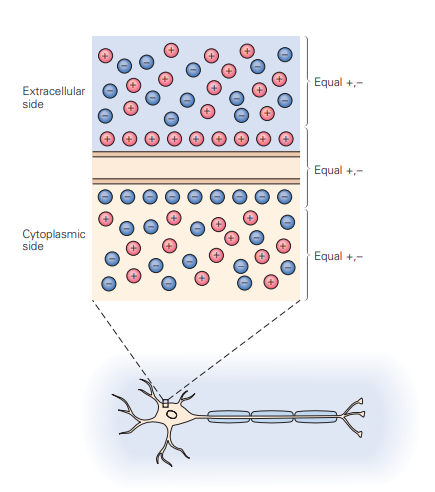
\includegraphics[width=0.6\textwidth]{resting_membrane_potential.png}
    \caption{Resting membrane potential (Source: Principles of Neural Science\cite{principles_of_neural_science})}
    \label{fig:resting_membrane_potential}
\end{figure}

\subsubsection{Generation of Action Potentials}

Action potentials, the transient electrical signals responsible for rapid communication within the nervous system, are generated when the membrane potential depolarizes beyond a certain threshold. This depolarization is initiated by the opening of voltage-gated sodium channels in response to a stimulus. As Na+ ions rush into the cell, the membrane potential becomes more positive, reaching around +40 mV.

\subsubsection{Propagation of Action Potentials}

Once initiated, the action potential propagates along the axon of the neuron. This propagation occurs through a self-regenerating process where the depolarization of one region of the membrane triggers the opening of voltage-gated sodium channels in the adjacent region, leading to further depolarization. This continues along the length of the axon, allowing the action potential to travel rapidly towards the synapse.

\subsubsection{Repolarization and Hyperpolarization}

Following depolarization, the membrane potential undergoes repolarization, returning to its resting state. This repolarization is driven by the opening of voltage-gated potassium channels, allowing K+ ions to exit the cell, while voltage-gated sodium channels undergo inactivation. In some cases, repolarization may overshoot, leading to hyperpolarization, before eventually returning to the resting membrane potential\cite{principles_of_neural_science}.

\section{Formulation of the Hodgkin-Huxley Model}

The Hodgkin-Huxley model provides a quantitative description of membrane currents and their role in nerve conduction and excitation. Central to this model is the representation of the neuronal membrane as an electrical circuit, which captures the dynamics of ion flow across the membrane during the generation and propagation of action potentials.

\begin{figure}[htbp]
    \centering
    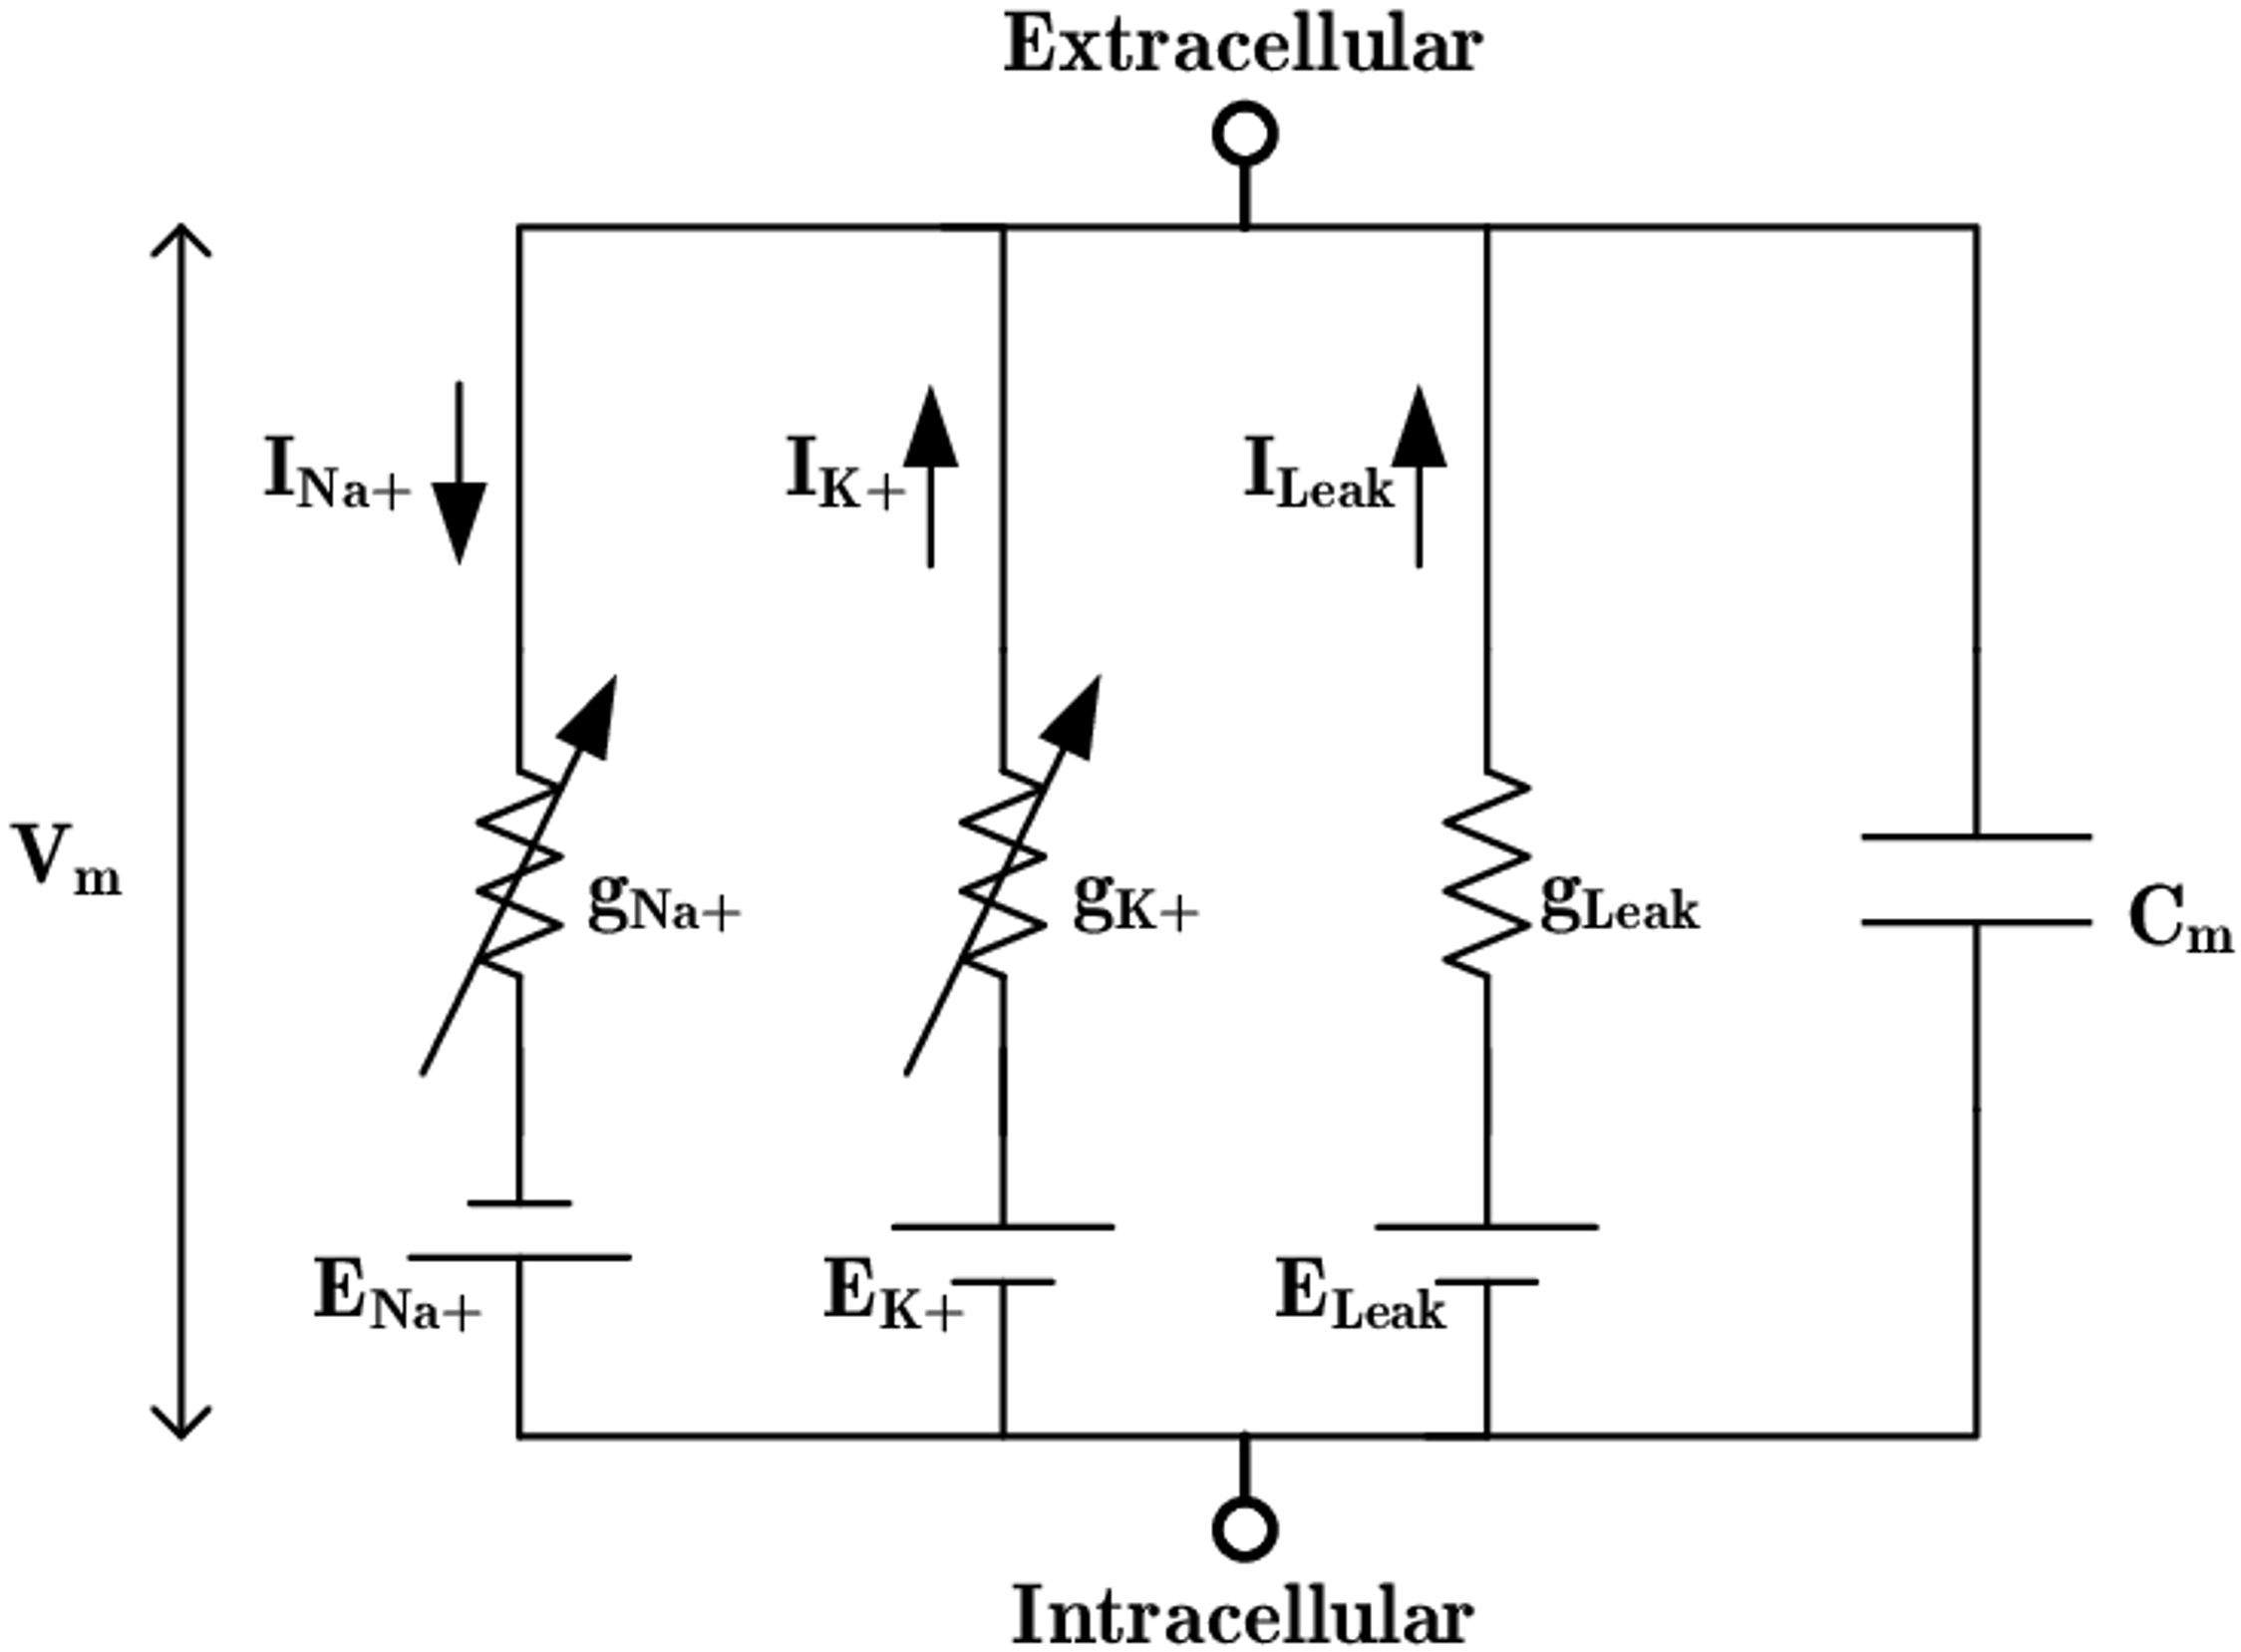
\includegraphics[width=0.6\textwidth]{electrical_circuit_representing membrane.png}
    \caption{Electrical circuit representing membrane. (Source: A quantitative description of membrane current and its application to conduction and excitation in nerve\cite{Hodgkin1952})}
    \label{fig:electrical_circuit_representing membrane.}
\end{figure}

\subsection{Electrical Circuit Representation}

In the Hodgkin-Huxley model, the neuronal membrane is represented as an electrical circuit composed of several components.

Membrane Capacitance (C): The lipid bilayer of the neuronal membrane acts as a capacitor, storing charge and contributing to the membrane's ability to maintain a voltage gradient.

Ion Channels: Voltage-gated ion channels, including sodium (Na+), potassium (K+), and leak channels, are represented as resistors in the circuit. These channels control the flow of ions across the membrane in response to changes in membrane potential.

Battery (Em): The battery in the circuit represents the resting membrane potential, which is typically around -60 to -70 mV in neurons. It serves as the reference voltage against which changes in membrane potential are measured.

\subsection{The Hodgkin-Huxley Equation}

The Hodgkin-Huxley model provides a quantitative description of membrane current and its application to conduction and excitation in nerve cells. It represents the dynamic interplay of ion channels and membrane capacitance in generating and propagating action potentials.

The model is formulated based on the principles of electrical circuits. The total current in the neuron can be expressed as the sum of the individual ion currents and the capacitive current:
\[
I_{\text{Total}} = I_{\text{Na}} + I_{\text{K}} + I_{\text{leak}} + I_{\text{C}}
\]

Using the relationship between charge ($Q$), capacitance ($C$), and potential difference ($V$):
\[
C = \frac{Q}{V}
\]

We can express the capacitive current ($I_C$) as the rate of change of charge with respect to time:
\[
C \frac{dV}{dt} = I_{\text{Total}} - I_{\text{Na}} - I_{\text{K}} - I_{\text{leak}}
\]

Applying Ohm's law ($I = \frac{V}{R}$), where $R$ is the resistance, to each ion current:
\[
I = \frac{1}{R} \times V
\]

We can modify this to incorporate the reversal potential ($E$):
\[
I = \frac{1}{R} \times (V - E)
\]

Substituting these into the equation for the capacitive current:
\[
C \frac{dV}{dt} = I_{\text{Total}} - \frac{1}{R_{\text{Na}}} \times (V_m - E_{\text{Na}}) - \frac{1}{R_{\text{K}}} \times (V_m - E_{\text{K}}) - \frac{1}{R_{\text{leak}}} \times (V_m - E_{\text{leak}})
\]

Where $V_m$ represents the membrane potential, and $E_{\text{Na}}$, $E_{\text{K}}$, and $E_{\text{leak}}$ represent the equilibrium potentials for sodium, potassium, and leak currents respectively.

Expanding the equation using the Hodgkin-Huxley model for the conductance of each ion ($g$) and the gating variables ($m$, $h$, $n$):
\begin{align*}
C \frac{dV}{dt} & = I_{\text{Total}} - g_{\text{Na}} m^3 h (V_m - E_{\text{Na}}) \\
                 & \quad - g_{\text{K}} n^4 (V_m - E_{\text{K}}) - g_{\text{leak}} (V_m - E_{\text{leak}})
\end{align*}

Where
\[
\frac{dm}{dt} = -\frac{(m - m_{\infty}(V))}{\tau_m(V)}, \quad \frac{dh}{dt} = -\frac{(h - h_{\infty}(V))}{\tau_h(V)}, \quad \frac{dn}{dt} = -\frac{(n - n_{\infty}(V))}{\tau_n(V)}
\]
represent the gating variable dynamics.

\begin{itemize}
  \item The equation $\frac{dm}{dt} = -\frac{(m - m_{\infty}(V))}{\tau_m(V)}$ represents the dynamics of the gating variable $m$. 
  \begin{itemize}
    \item $m$ represents the activation gating variable for sodium channels.
    \item $m_{\infty}(V)$ is the steady-state value of $m$ at membrane potential $V$, which describes the fraction of sodium channels that are open.
    \item $\tau_m(V)$ is the time constant associated with the activation gating variable $m$, which determines how quickly $m$ changes with respect to time.
  \end{itemize}
  
  \item Similarly, the equation $\frac{dh}{dt} = -\frac{(h - h_{\infty}(V))}{\tau_h(V)}$ represents the dynamics of the gating variable $h$.
  \begin{itemize}
    \item $h$ represents the inactivation gating variable for sodium channels.
    \item $h_{\infty}(V)$ is the steady-state value of $h$ at membrane potential $V$, which describes the fraction of sodium channels that are inactivated.
    \item $\tau_h(V)$ is the time constant associated with the inactivation gating variable $h$, determining how quickly $h$ changes over time.
  \end{itemize}
  
  \item Finally, the equation $\frac{dn}{dt} = -\frac{(n - n_{\infty}(V))}{\tau_n(V)}$ represents the dynamics of the gating variable $n$.
  \begin{itemize}
    \item $n$ represents the activation gating variable for potassium channels.
    \item $n_{\infty}(V)$ is the steady-state value of $n$ at membrane potential $V$, indicating the fraction of potassium channels that are open.
    \item $\tau_n(V)$ is the time constant associated with the activation gating variable $n$, governing how quickly $n$ changes with time.
  \end{itemize}
\end{itemize}

These equations describe how the gating variables $m$, $h$, and $n$ change over time in response to changes in membrane potential $V$. They play a crucial role in determining the conductance of sodium and potassium channels, which, in turn, influences the generation and propagation of action potentials in neurons\cite{Hodgkin1952}.


\section{Python Simulation}

This section presents the results of the simulation using the Hodgkin-Huxley model for different applied external currents. The simulation was conducted to understand the behavior of the neuron in response to varying input stimuli and to validate the model against known physiological phenomena.

\subsection{Simulation Results}
The Hodgkin-Huxley model explains how the dynamics of ion channels (Na+, K+ etc) contribute to the generation of an Action Potential in a neuron.
An Action Potential is a sharp voltage spike elicited by stimulating a neuron with a current
that exceeds a certain threshold value. The current amplitude is increased gradually, at a
threshold amplitude, the voltage response does not increase proportionally.
It shows a sharp, disproportionate increase.
Once the membrane voltage reaches a threshold value, it increases further rapidly to maximum value and drops again rapidly to a value that is less than resting value, before returning
to the baseline value after a delay.


\begin{itemize}
  \item For input currents ranging from 0µA to 0.02235µA, no action potentials were observed.
\end{itemize}

\begin{figure}[htbp]
    \centering
    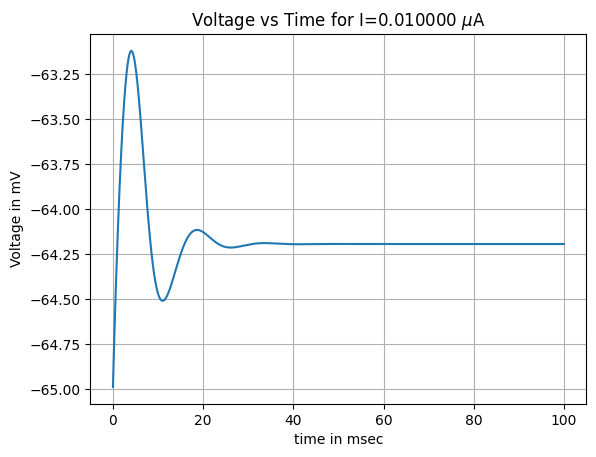
\includegraphics[width=0.6\textwidth]{voltage_time_0_01uA.png}
    \caption{Plot of Voltage vs Time for I=0.01µA}
    \label{fig:voltage_time_0_01uA}
\end{figure}

\begin{figure}[htbp]
    \centering
    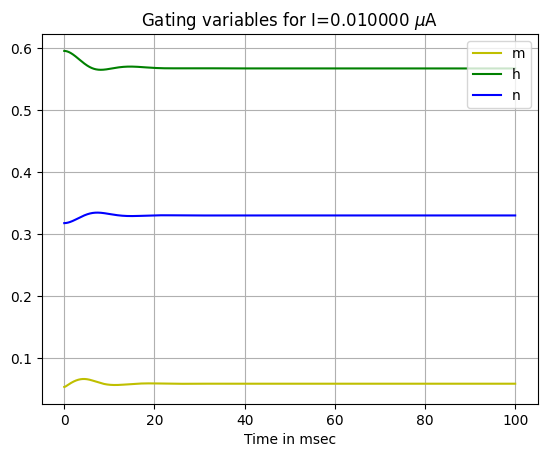
\includegraphics[width=0.6\textwidth]{gating_variables_0_01uA.png}
    \caption{Plot of gating variables for I=0.01µA}
    \label{fig:gating_variables_0_01uA}
\end{figure}

\begin{figure}[htbp]
    \centering
    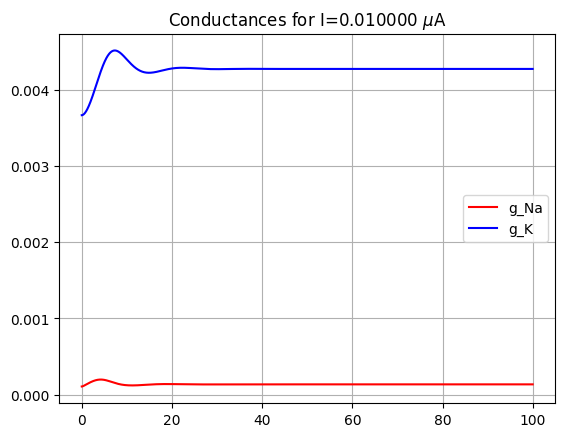
\includegraphics[width=0.6\textwidth]{conductances_0_01uA.png}
    \caption{Plot of conductances for I=0.01µA}
    \label{fig:conductances_0_01uA}
\end{figure}

\begin{itemize}
  \item A sudden onset of action potentials occurred when the input current was increased from 0.02235µA to 0.02236µA. However, these action potentials were not periodic.
\end{itemize}

\begin{figure}[htbp]
    \centering
    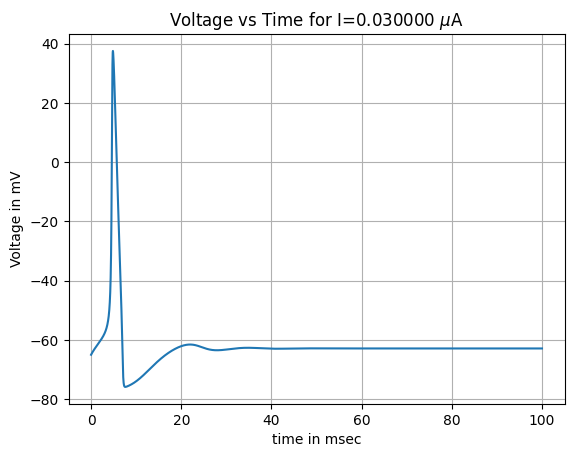
\includegraphics[width=0.6\textwidth]{voltage_time_0_03uA.png}
    \caption{Plot of Voltage vs Time for I=0.03µA}
    \label{fig:voltage_time_0_03uA}
\end{figure}

\begin{figure}[htbp]
    \centering
    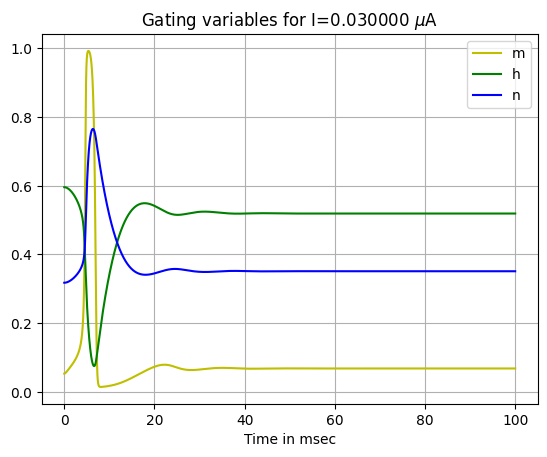
\includegraphics[width=0.6\textwidth]{gating_variables_0_03uA.png}
    \caption{Plot of gating variables for I=0.03µA}
    \label{fig:gating_variables_0_03uA}
\end{figure}

\begin{figure}[htbp]
    \centering
    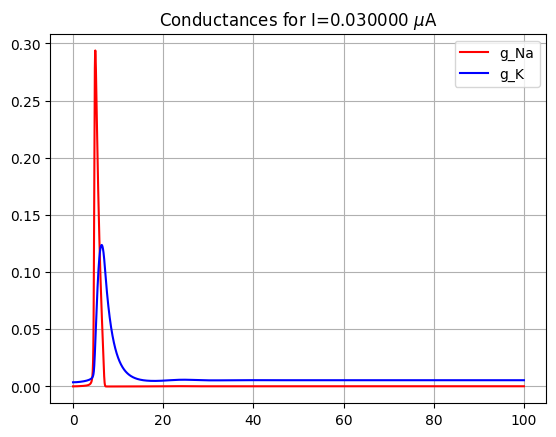
\includegraphics[width=0.6\textwidth]{conductances_0_03uA.png}
    \caption{Plot of conductances for I=0.03µA}
    \label{fig:conductances_0_03uA}
\end{figure}

\begin{itemize}
  \item Periodic action potentials were observed when the input current was further increased from 0.0622µA to 0.06223µA.
\end{itemize}

\begin{itemize}
  \item For input currents ranging from 0.06223µA to 0.450µA, periodic action potentials were observed.
\end{itemize}

\begin{figure}[htbp]
    \centering
    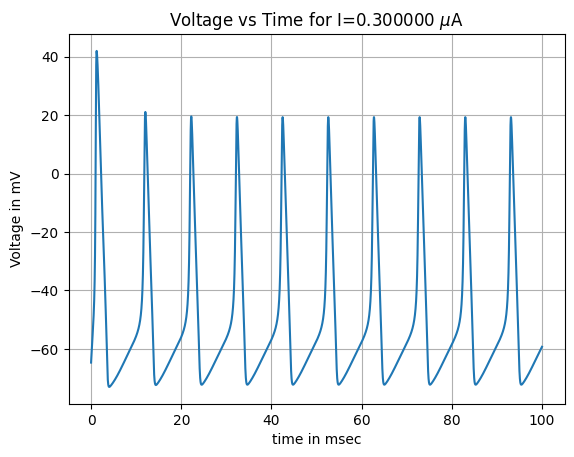
\includegraphics[width=0.6\textwidth]{voltage_time_0_3uA.png}
    \caption{Plot of Voltage vs Time for I=0.3µA}
    \label{fig:voltage_time_0_3uA}
\end{figure}

\begin{figure}[htbp]
    \centering
    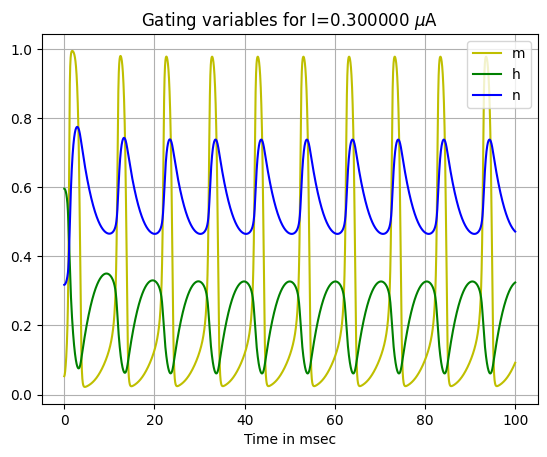
\includegraphics[width=0.6\textwidth]{gating_variables_0_3uA.png}
    \caption{Plot of gating variables for I=0.3µA}
    \label{fig:gating_variables_0_3uA}
\end{figure}

\begin{figure}[htbp]
    \centering
    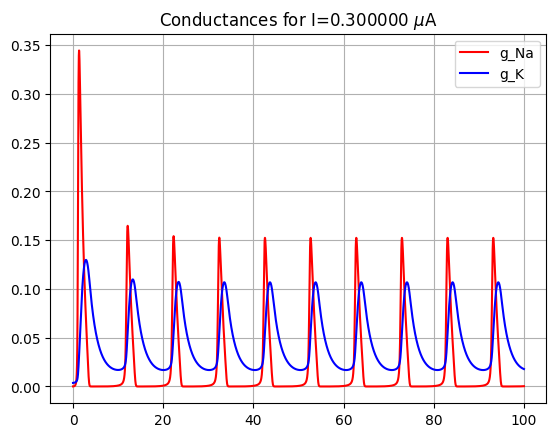
\includegraphics[width=0.6\textwidth]{conductances_0_3uA.png}
    \caption{Plot of conductances for I=0.3µA}
    \label{fig:conductances_0_3uA}
\end{figure}

\begin{itemize}
  \item Action potentials ceased when the input current was increased beyond 0.450µA.
\end{itemize}

\begin{figure}[htbp]
    \centering
    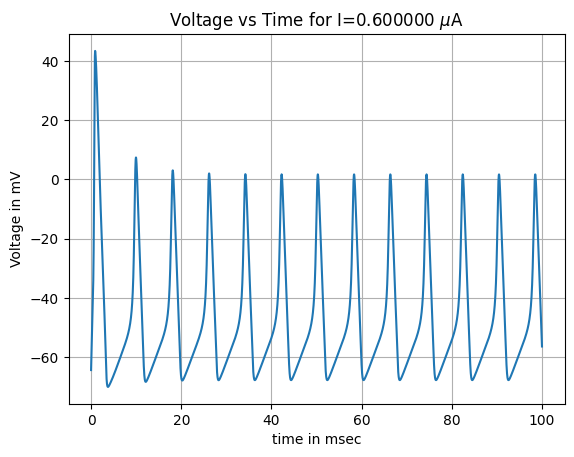
\includegraphics[width=0.6\textwidth]{voltage_time_0_6uA.png}
    \caption{Plot of Voltage vs Time for I=0.6µA}
    \label{fig:voltage_time_0_6uA}
\end{figure}

\begin{figure}[htbp]
    \centering
    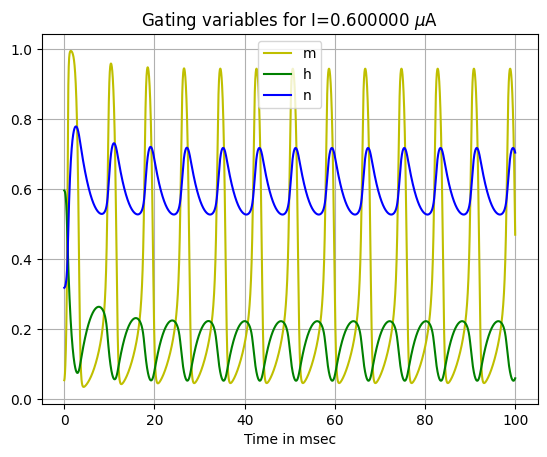
\includegraphics[width=0.6\textwidth]{gating_variables_0_6uA.png}
    \caption{Plot of gating variables for I=0.6µA}
    \label{fig:gating_variables_0_6uA}
\end{figure}

\begin{figure}[htbp]
    \centering
    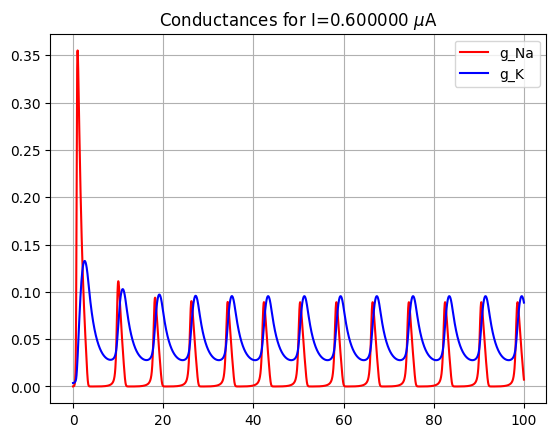
\includegraphics[width=0.6\textwidth]{conductances_0_6uA.png}
    \caption{Plot of conductances for I=0.6µA}
    \label{fig:conductances_0_6uA}
\end{figure}





\begin{thebibliography}{9}
\bibitem{Cole1939} Cole, K. S., Curtis, H. J. Electric impedance of the squid giant axon during activity. Journal of General Physiology, 22(5), 649–670 (1939). 
\url{https://doi.org/10.1085/jgp.22.5.649}
\bibitem{Hodgkin1939}HODGKIN, A., HUXLEY, A. Action Potentials Recorded from Inside a Nerve Fibre. Nature 144, 710–711 (1939).
\url{https://doi.org/10.1038/144710a0}
\bibitem{Hodgkin1949} Hodgkin, A. L., Katz, B. (1949). The effect of sodium ions on the electrical activity of the giant axon of the squid. The Journal of Physiology, 108. 
\url{https://doi.org/10.1113/jphysiol.1949.sp004310}
\bibitem{Hodgkin1952} Hodgkin, A. L., Huxley, A. F., (1952), A quantitative description of membrane current and its application to conduction and excitation in nerve. The Journal of Physiology, 117 
\url{https://doi: 10.1113/jphysiol.1952.sp004764}
\bibitem{Hausser2000} Häusser, M. The Hodgkin-Huxley theory of the action potential. Nat Neurosci 3 (Suppl 11), 1165 (2000). \url{https://doi.org/10.1038/81426}
\bibitem{principles_of_neural_science}
Kandel, E. R., Schwartz, J. H., Jessell, T. M., Siegelbaum, S. A., Hudspeth, A. J. (2014). Principles of Neural Science (5th ed.). McGraw-Hill Education. ISBN: 978-0-07-181001-2.

\end{thebibliography}

\end{document}
